%!TEX root = ../thesis.tex
\chapter{Methods}
\label{ch:methods}

\todo{approach section, use model project overview graphic (?)}
The key idea of our approach is to use the versatile MATLAB platform to create an easily expandable model of a hexapod robot, aiming to accelerate future research.
By basing our work on this platform we will in the future be able to incorporate concepts from different domains with a more streamlined development process and less development time, given the provided toolboxes.
In this chapter we detail the approach and methodology used to address the objectives we defined in the introduction.
As the controller and RL setup both depend on a solid, well-working model, we will first describe the representation of the hexapod we created in Simulink.
We will then continue with a description of the static gait motion controller, including trajectory generation and inverse kinematics solver.
The chapter concludes with the explanation of our reinforcement learning setup used to train an agent on leg coordination/ gait generation.


\section{Simulink Model}
\todo{Intro for Simulink model}

\begin{figure}[h]
	\centerline{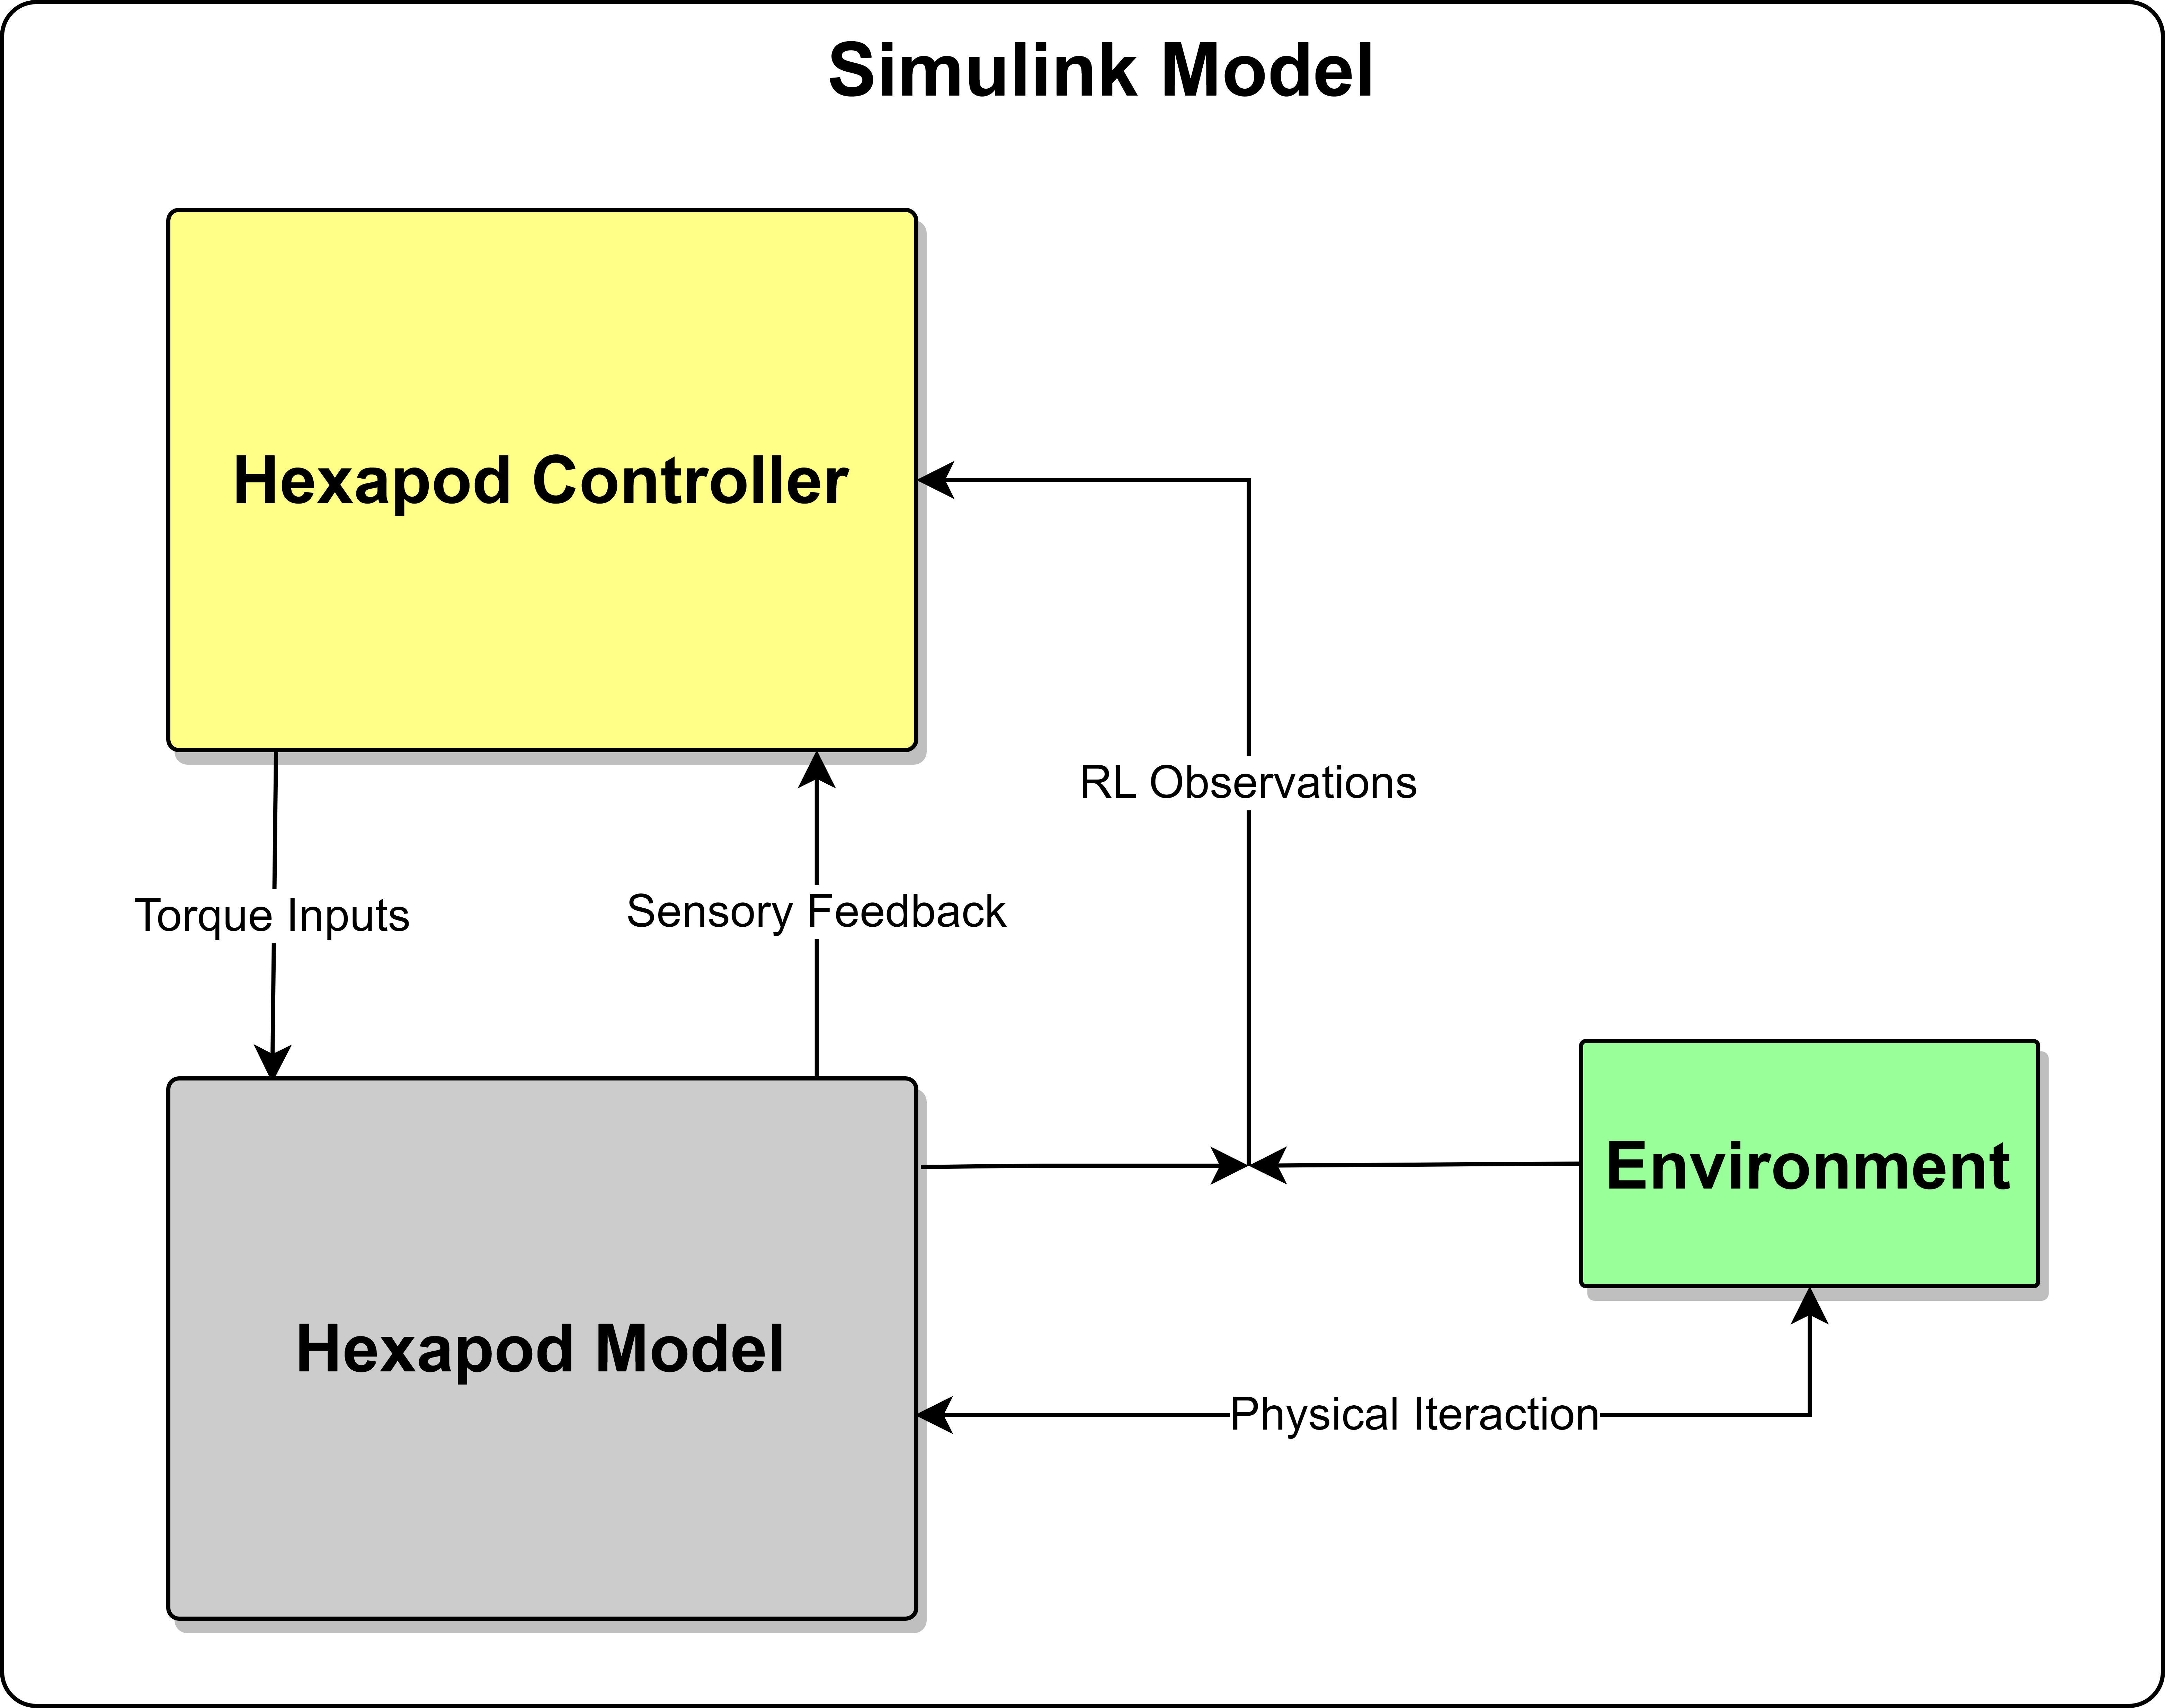
\includegraphics[scale=0.035]{HexapodModel_Overview}}
	\caption{Simulink Model Overview}
	\label{figure: Simulink Model Overview}
\end{figure}

\subsection{Model of the Hexapod}
The hexapod model we develop in this thesis is based on the \textit{PhantomX MK4} hexapod distributed by \textit{Trossen Robotics}.
The company provides a digital model of this robot in the form of an .urdf file which can be obtained from their Github page \parencite{interboticsGithub}.
URDF (\textbf{U}nified \textbf{R}obotics \textbf{D}escription \textbf{F}ormat) is a common file format for describing the physical and kinematic properties of a robot or robotic component.
It provides a standardized and structured way to define the connections between joints and links, the visual properties and collision geometry of each link as well as parameters such as mass and inertia \parencite{matlabURDFDocumentation}.
The geometry is provided in a separate folder in the form of CAD-files which are then referenced by the urdf.

The \textit{PhantomX MK4} follows the common architecture mentioned in \ref{sec: Hexapods}, meaning each leg has 3 joints and segments, totalling 18 DoFs.
Concerning the joint orientations, the \textalpha-joints movement plane lies is parallel to the ground while the \textbeta- and \textgamma-joint are restricted to a plane perpendicular to the ground, also in accordance to mentioned architecture.
The robot is axisymmetric towards its central axis(pointing in the movement direction) and the front and hind leg pairs are equally spaced from the middle leg pair.
The middle legs are attached to the thorax slightly further away from the central axis than the front and back legs.
A 3D model of the hexapod can be seen in Fig. \ref{figure: PhantomX 3D model}.

To import the model into the Simulink environment, we us a MATLAB-provided function to convert it from a urdf-file into a Simulink block diagram.
This process works automatically and results in a physically accurate Simulink representation without having to manually re-model the robot.
The representation consists of blocks from the Simscape library, more specifically joints, rigid transforms and coordinate frames to describe the robots kinematic chains, and rigid bodies to represent the individual links geometry and physical parameters.

\begin{figure}[h]
	\begin{subfigure}{.5\textwidth} % this sets the figure to be max half the width of the page
		\centering
		% include first image
		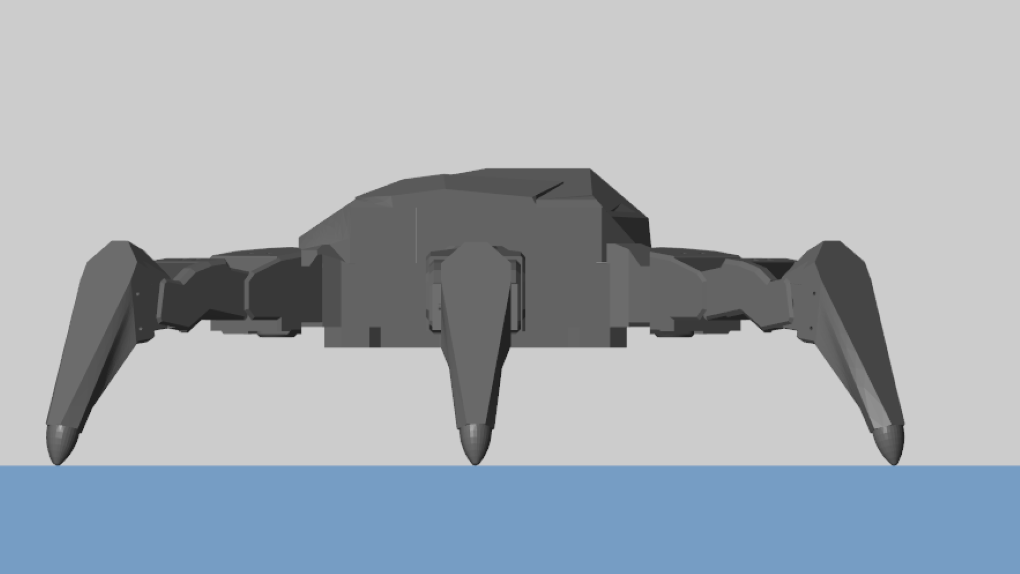
\includegraphics[width=.9\linewidth]{PhantomX_MK4_SideView}  % this sets the image to fill 90% of the available space -> 45% of the line width in total. 
		\caption{}
		\label{figure: PhantomX Side View}
	\end{subfigure}
	\begin{subfigure}{.5\textwidth}
		\centering
		% include second image
		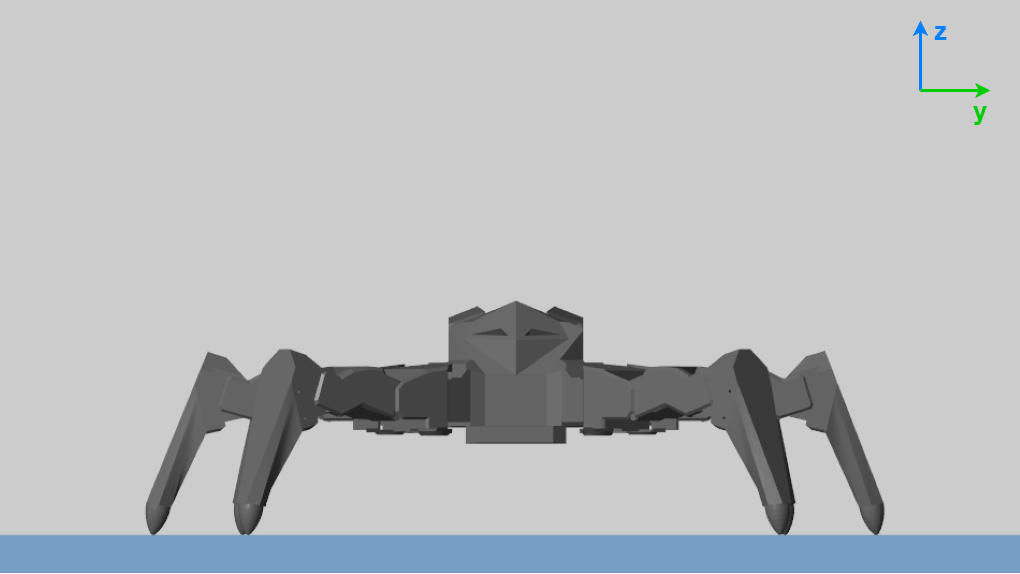
\includegraphics[width=.9\linewidth]{PhantomX_MK4_FrontView}  
		\caption{}
		\label{figure: PhantomX Front View}
	\end{subfigure}
	
	\label{fig:fig}
	\begin{subfigure}{\textwidth}
		\centering
		% include third image
		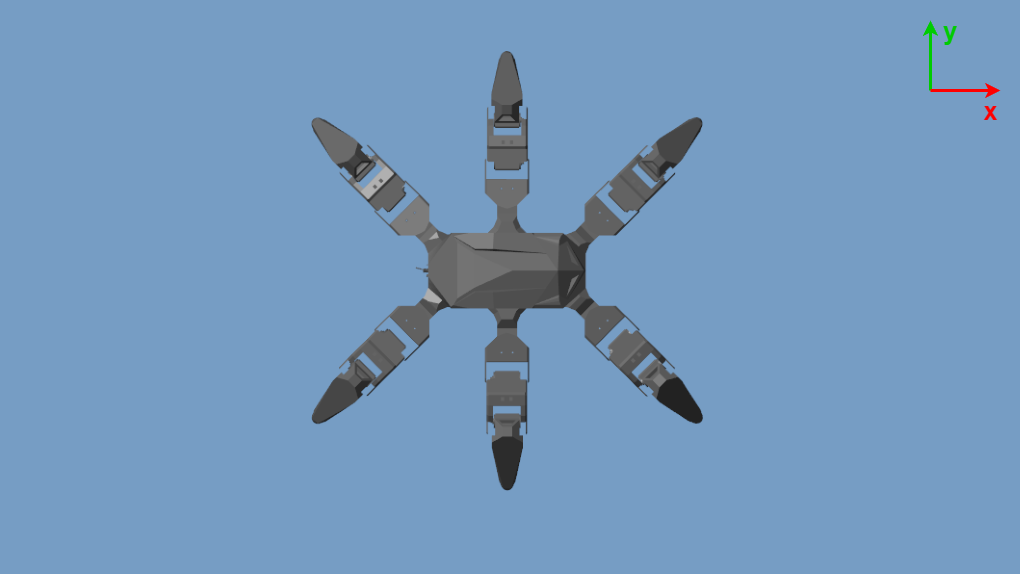
\includegraphics[width=.45\linewidth]{PhantomX_MK4_TopView}   % this width should be half of the width of the other two images
		\caption{}
		\label{figure: PhantomX Top View}
	\end{subfigure}
	\caption[]{3D model of Trossen Robotics PhantomX MK4}
	\label{figure: PhantomX 3D model}
\end{figure}
\todo{get each image into list of figures, but exclude complete figure}

To be able to use the imported hexapod as a development platform we have to modify and expand the raw Simulink model as it does not provide any means to control it or receive feedback.
We reorganise and encapsulate logical groups, specifically the thorax and the individual legs, into library subsystems.
This enables us to propagate changes faster, as we only have to edit the library component instead of each existing instance.
As a side effect, this given the Simulink model a much more cleaned up and easier to understand appearance.
To be able to control each joint and receive sensory feedback from it, we enable the so called \textit{direct torque input} as well as the \textit{position} and \textit{acceleration} sensor readings on each joint block.
Trying to prevent increasing the models complexity to quickly, we do not model the physical servo motor attached to each joint and instead use the instantaneous torque application.
the joint block also allows for physical parameters to be modified, such as internal friction, dampening or spring stiffness.
We combine the 3 torque values and position/ acceleration readings of each leg into an input and output bus signal.
A view inside of the leg subsystem is given in \ref{figure: Hexapod Leg}, the subsystem block itself with its torque input and sensory feedback output buses can be seen in \ref{figure: Hexapod Model Overview} as part of the complete hexapod model.

\begin{figure}[h]
	\centerline{\includesvg[scale=0.55]{Simulink/Simulink_PhysicalHexapodOverview}}
	\caption{Overview of the Simulink Hexapod Model}
	\label{figure: Hexapod Model Overview}
\end{figure}

\begin{figure}
	\centerline{\includesvg[scale=0.5]{Simulink/Simulink_HexapodLegOverview}}
	\caption{Simulink model of the Hexapod Leg subsystem}
	\label{figure: Hexapod Leg}
\end{figure}

To enable the robot to physically interact with its surroundings, we enable the collision geometry on each of the models rigid bodies.
In Simscape, collision modelling involves establishing connections between a rigid body, and any other rigid body it should be able to interact with in a collision scenario, via Simscapes's \textit{Spatial friction force} block.
The block allows to modify the coefficients of static and dynamic friction, elasticity and dampening.\todo{does dampening exist in block ?}
An example of how this block can be utilized is shown in \ref{figure: Simscape Bouncing Ball Example}.
As collision detection is computationally relative expensive, we refrain from modelling robot self collisions and focus only on the interaction between robot and environment.
This means that the hexapods links can only collide with the ground plane but not with each other.
We realise this can potentially create discrepancies between simulation and real world, but as we initially only model predefined leg trajectories, which can be proven to not intersect, we are willing to give up a bit of realism in favour of faster simulations.

From a top level perspective, the modified robot model is represented by a single \textit{Hexapod} subsystem block, which receives the torques to be applied as input and outputs sensory information about each joint.
All of the internal joint parameters and friction coefficients used to model collisions are given in the tables \ref{table: Joint parameters} and \ref{X}.
The joint parameters were already mostly given by the urdf specification, while we adapted other parameters from \parencite{AUTHOR} and \parencite{AUTHOR2}.
\todo{Find source again}
To summarize, we converted the provided hexapod model into a Simulink model, compartmentalized it and added sensing and actuation capabilities to the robots legs.
In addition we made most of the models internal parameters accessible and modifiable within the MATLAB-script \textit{simulationsetup.m}.



\begin{comment}
The  thorax is represented by a rigid body and a main coordinate frame.
Each of the robots legs consists of 3 rigid bodies(coxa, femur and tibia) which are connected to each other by 2 joints.
A third joint then attaches the coxa and the leg as a whole to the main body.
Like the leg of an insect, the movement plane of the joint connecting coxa and thorax is parallel to the ground and orthogonal towards the other two joints.
Each of the joints used has 1 (rotational) DoF.
To position each rigid body and joint correctly, rigid transformations are used to translate and rotate each component.

As mentioned above, joints can receive as input a torque to be applied and can output sensory data, such as the joints position, velocity and acceleration. 
\end{comment}


\begin{table}
	\centering
	\begin{tabular}{| l | c |}
		\hline
		\textbf{parameter} & \textbf{value} \\
		\hline
		spring stiffness & 0 \\
		\hline
		damping coefficient & 0 \\
		\hline
		spring stiffness(joint boundary) & $10^4 \frac{Nm}{\text{deg}}$ \\
		\hline
		damping coefficient(joint boundary) &  $10 \frac{Nm \cdot s}{\text{deg}}$\\
		\hline
		transit region width(joint boundary) &  $10^{\circ}$\\
		\hline
	\end{tabular}
	\caption{Internal joint parameters}
	\label{table: Joint parameters}
\end{table}


%In this thesis we only utilize the sensor information about the current joint positions, but to allow for further expansions on the model, such as optimizing for minimal energy consumption, joint velocity and acceleration are provided as well.
%It should be noted, that integrating the joint position over time would implicitly yield the same result, but we decided for ease of use to include this data explicitly.


\subsection{Environment}
To validate the robot model and to provide a place for the robot to learn the coordination rules of its legs, we constructed a simple test environment.
The environment currently only consists of a horizontal plane, but can expanded to include more complex terrain with little effort.
Some examples which we experimented with but did not include in this thesis are inclined planes and also small obstacles on the ground.
As Simscape itself only provides basic geometric objects but allows for the use .stl files to define the shape of objects, complex terrain such as irregular, uneven surfaces can be imported with relative ease.

In addition to being the testing ground of the hexapod model, the environment also acts as part of the reinforcement learning process.
Similar to \ref{figure: RL Illustration}, the environment provides observations to the RL agent and calculates a reward signal, based on the agents performance.
It does not directly receive actions from the agent, as the hexapod to which the actions are applied is its own subsystem.
If we would define the environment exactly like \ref{figure: RL Illustration,}, we would have to include both the environment subsystem and the hexapod subsystem as part of the "RL" environment.
For obvious reasons such as modularity and clarity of model we chose not to adapt this.

\subsection{Controller}
The controller is responsible for the hexapods locomotion.
It controls the movement of the robots six legs according to a predefined gait.
As inputs, the controller receives the sensory data from the hexapod model.
According to this data the controller outputs the torques to be applied to each joint.

\begin{figure}
	\centerline{\includegraphics[scale=0.03]{HexapodController}}
	\caption{Controller Overview}
	\label{figure: Controller Overview}
\end{figure}
As the legs will move independently from one another, each of the hexapods legs is controlled by a separate control unit.
These units receives information from the legs joint sensors as input and computes the torques to be applied to the joints as output.
A legs control unit receives the frequency for the swing-stance cycle, duty-percentage of the swing phase and swing-initiation signal as coordination inputs.
This information can either come from a static gait definition, in which the parameters for each leg are statically configured, or can be provided by a reinforcement learning agent.
The agent receives observations from the environment and hexapod model as well as a reward signal and outputs actions in the form as mentioned above.

\begin{figure}
	\centerline{\includesvg[scale=0.6]{Simulink/Simulink_LegControllerOverview}}
	\caption{Control unit for a single leg}
	\label{figure: Leg control unit}
\end{figure}

A single leg control unit, as seen in \ref{figure: Leg control unit}, consists of a leg trajectory generator and one PID feedback control loop for each of the 3 leg joints.
The leg trajectory generator is responsible for generating a path for the leg to follow according to the input frequency, duty cycle swing initiation and pattern rotation.
It outputs the desired angle for the \textalpha-, \textbeta- and \textgamma-joints, which the PID controllers are then trying to achieve.
The PID controller parameters $K_p$, $K_i$ and $K_d$ (and $N$) are tuned via trial-and-error method and are depicted in \ref{table: PID parameters}.

\begin{figure}
	\centerline{\includesvg[scale=0.75]{Simulink/Simulink_LegTrajectoryGenerationOverview}}
	\caption{Leg trajectory generator}
	\label{figure: Leg trajectory generator}
\end{figure}

The leg trajectory generator, as seen in \ref{figure: Leg trajectory generator}, consists of a signal generator, a pattern rotation subsystem and an analytic inverse kinematics solver.
The signal generator is responsible for creating a continuous leg trajectory in the form of 2-dimensional trajectory coordinates.
The pattern rotation subsystems the planar trajectory(x,z-plane), if required, around the z-axis to allow for omni-directional movement of the robot.
Finalizing the trajectory generation, the inverse kinematics solver receives the trajectory coordinates and translates them into joint angles.


\subsubsection{Analytical Inverse Kinematics Solver} \label{subsubsec: IK Solver}
Even though Simulinks \textit{Robotics System Toolbox} includes an iterative IK-solver, we decided to implement our own analytical solver.
Early in the development process, we realized that the iterative solver provided would not be sufficient for our intended purpose.
Due to the nature of iterative solution methods, the calculation time required to find a valid configuration is significantly higher than that of a purpose-build analytical solver and thus greatly increased simulation times.
As we need to simulate several thousand episodes during reinforcement learning, we aim to minimize the 
amount of time required to compute a time step in the simulation.

The solver sequentially calculates the 3 joint angles of a leg, starting at \textalpha, then \textbeta and \textgamma.
The solver is derived from the legs geometric properties as seen in \ref{figure: IK angle derivations}

\begin{figure}[h]
	\begin{subfigure}{.5\textwidth} % this sets the figure to be max half the width of the page
		\centering
		% include first image
		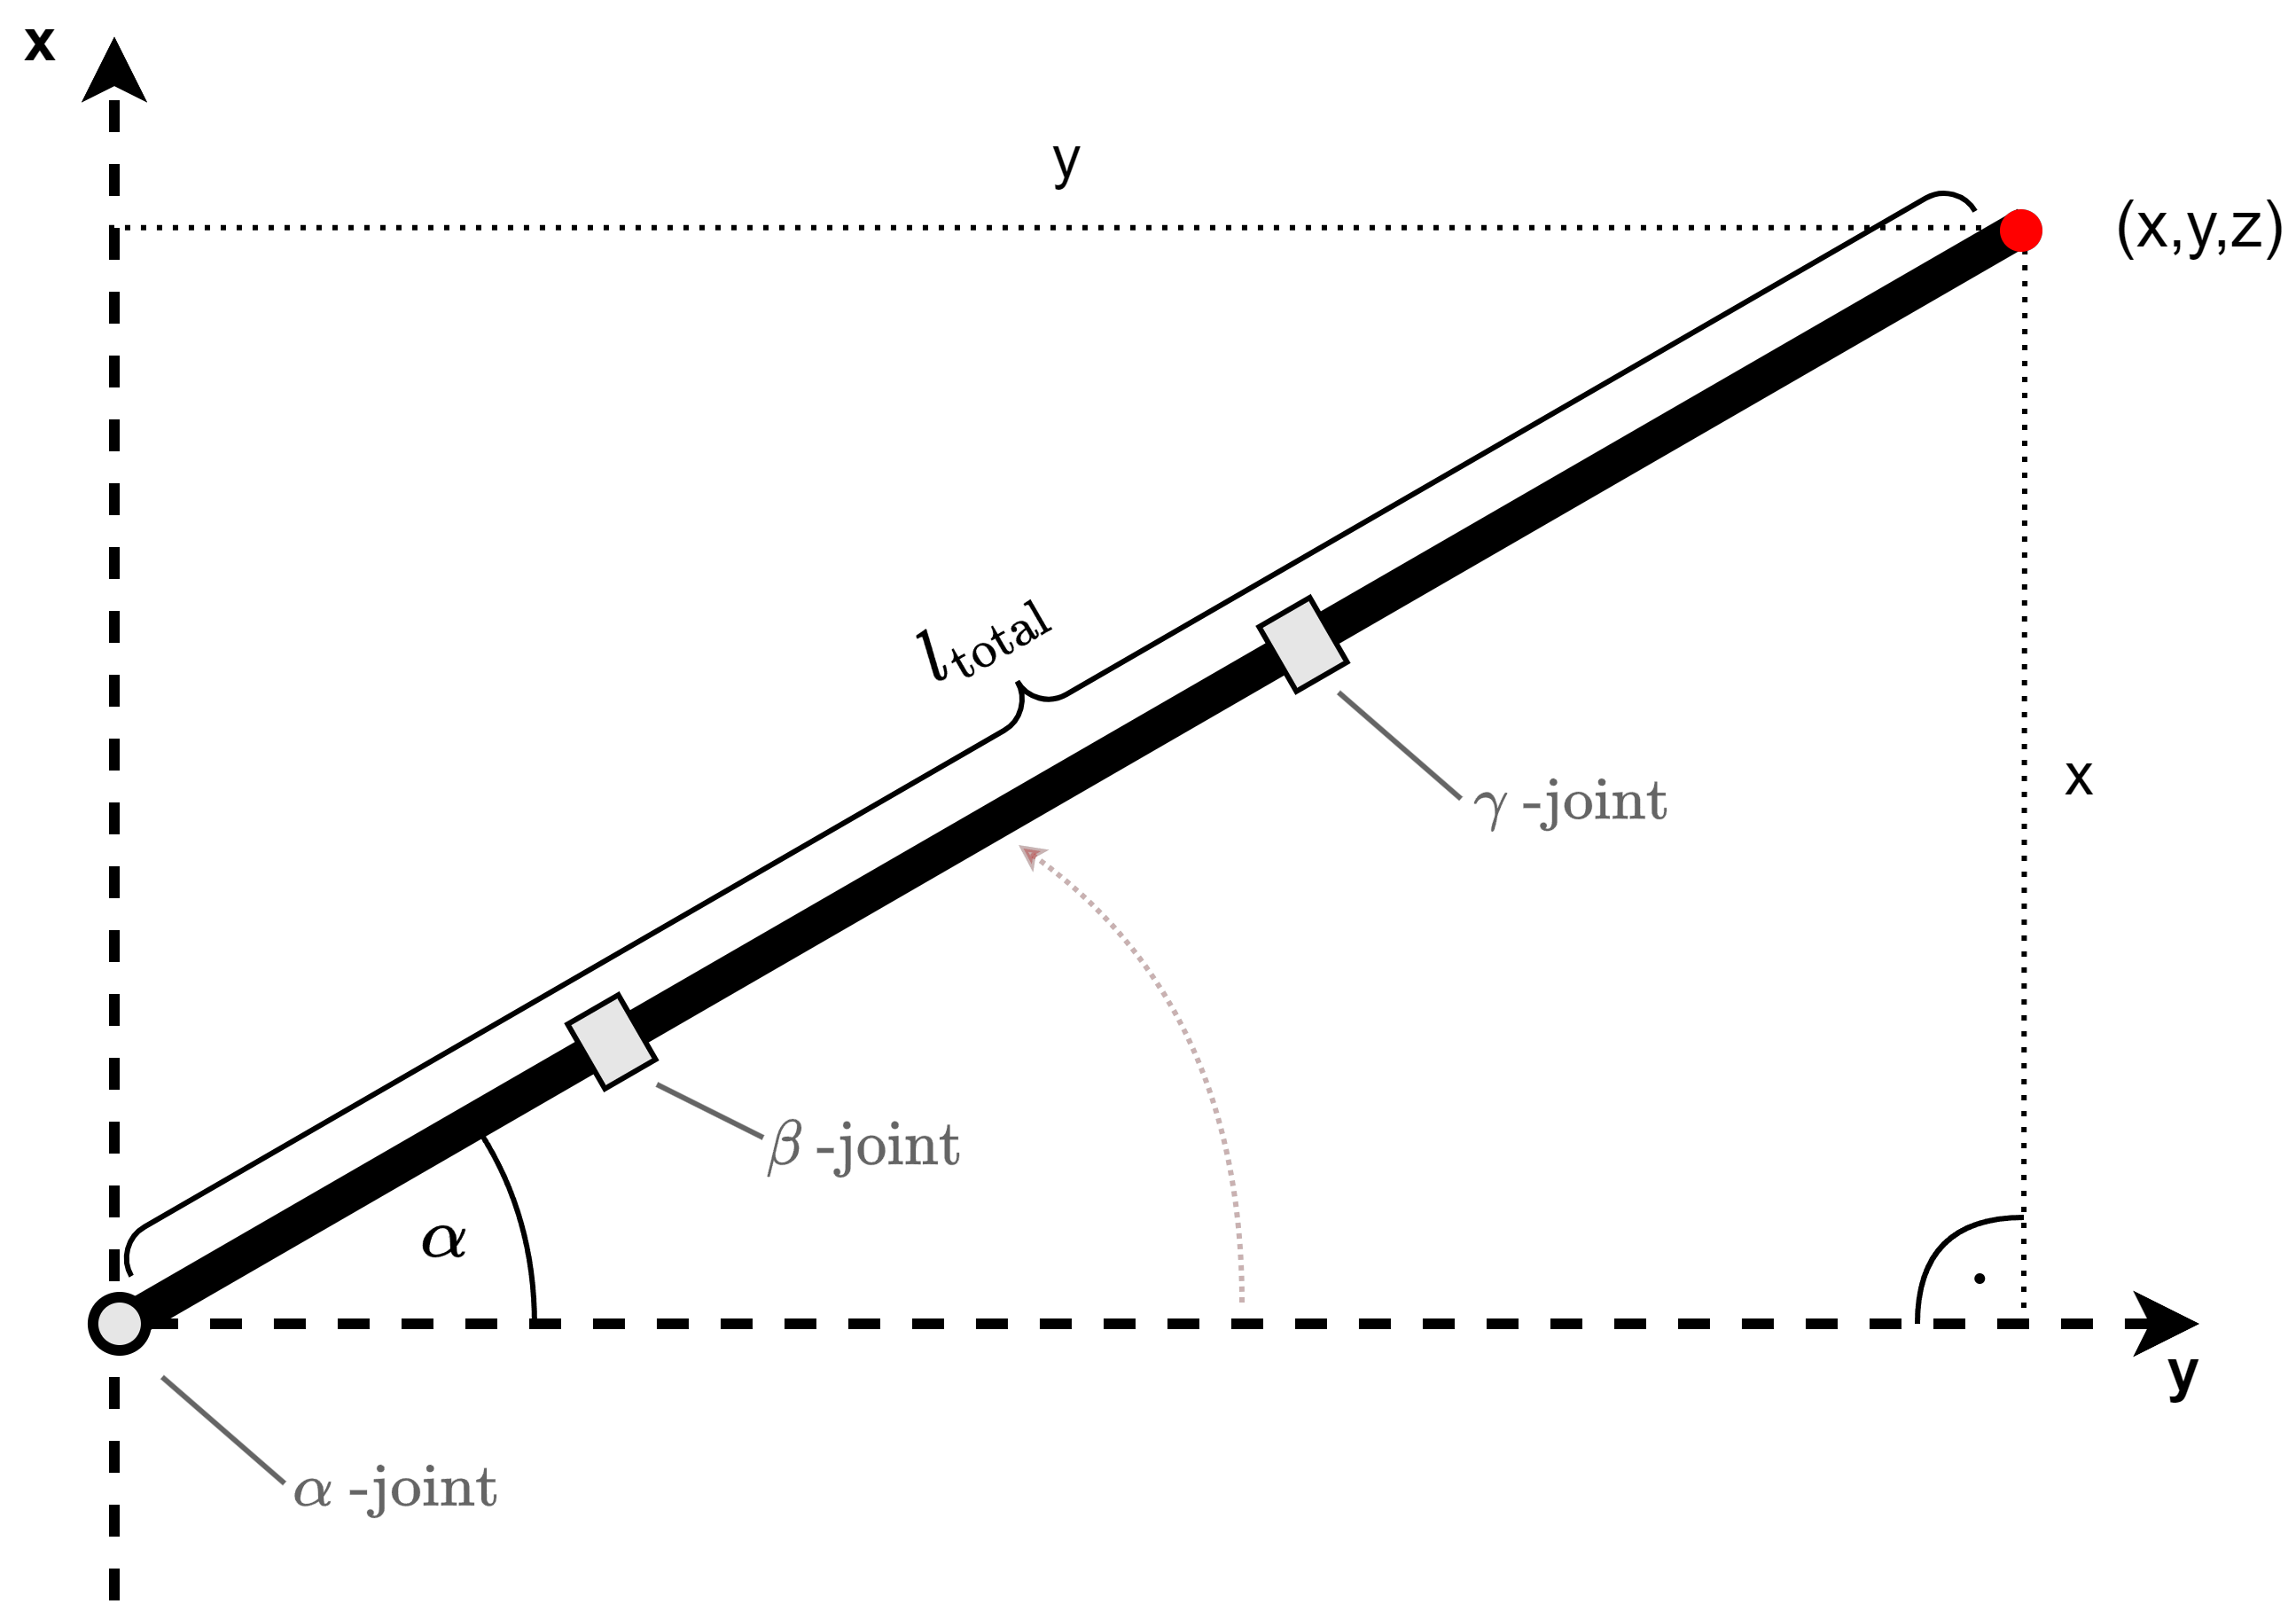
\includegraphics[width=\linewidth]{IK_Solver_alphaAngle}  % this sets the image to fill 90% of the available space -> 45% of the line width in total. 
		\caption{}
		\label{figure: IK Solver Alpha Angle}
	\end{subfigure}
	\begin{subfigure}{.5\textwidth}
		\centering
		% include second image
		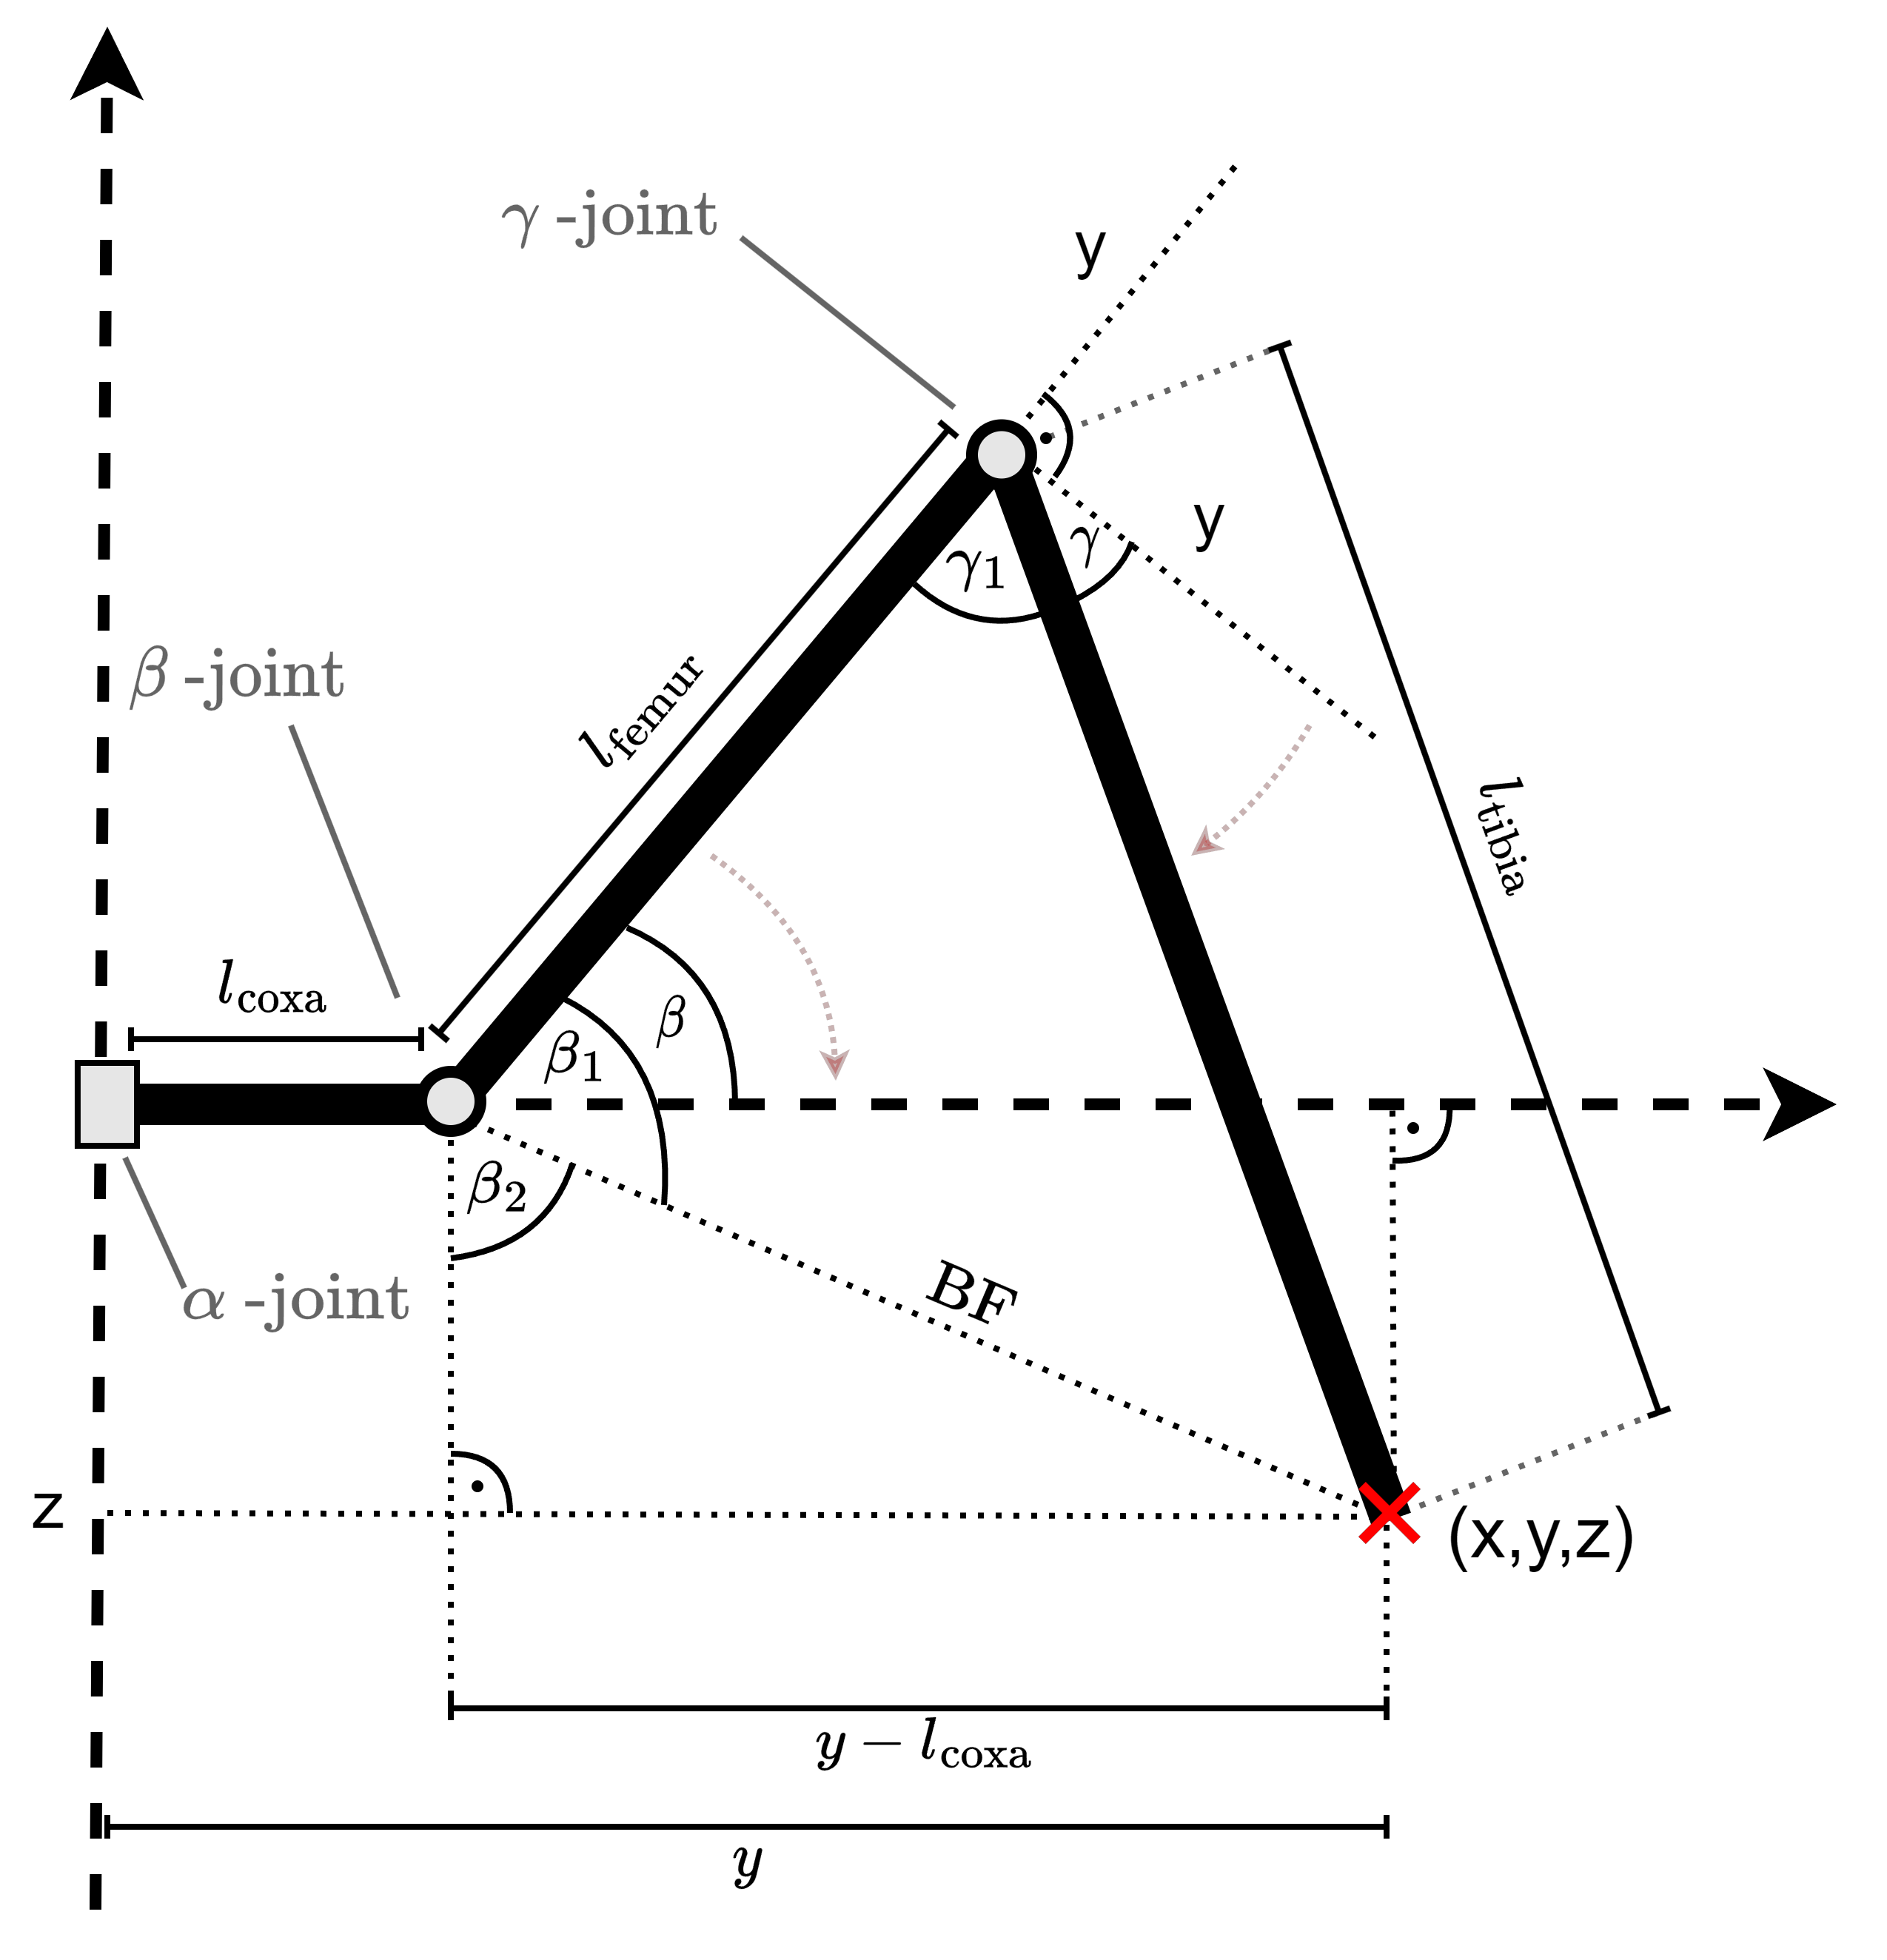
\includegraphics[width=\linewidth]{IK_Solver_betaGammaAngle}  
		\caption{}
		\label{figure: IK Solver Beta/Gamma Angle}
	\end{subfigure}
	\caption[Angle derivation drawings]{(a) Top-down view of a hexapod leg, used to determine \textalpha. (b) Side-view, used in the in the determination of \textbeta \ and \textgamma.}
	\label{figure: IK angle derivations}
\end{figure}


 Given the length of each leg segment, the 3 angles are calculated as following:

\[
	\alpha = \arctan(\frac{x}{y}) ,\quad \quad \quad \beta = 90^{\circ} - (\beta_1 + \beta_2) ,\quad \quad \quad \gamma = 90^{\circ} - \gamma_1.
\]
\\
Where $\beta_1$, $\beta_2$, $\gamma_1$ and \text{BF} are given by:
\[	
	\beta_1 = \arccos(\frac{{l_\text{femur}}^2 + \text{BF}^2 - {l_\text{tibia}}^2}  {2\cdot l_\text{femur} \cdot \text{BF}}) ,\quad \quad \quad \beta_2 = \arctan(\frac{ l_\text{total} - l_\text{coxa}} {z}),
\]

\[
	\gamma_1 = \arccos(\frac{{l_\text{tibia}}^2 + {l_\text{femur}}^2 - {\text{BF}}^2}  {2 \cdot {l_\text{tibia}} \cdot {l_\text{femur}}}) ,\quad \quad \quad \text{BF} = \sqrt{(l_\text{total} - l_\text{coxa})^2 + z^2}.
\]








\begin{figure}[h]
	\centerline{\includesvg[scale=0.85]{Simulink/Simulink_SignalGeneratorOverview}}
	\caption{Signal Generator}
	\label{figure: Signal Generator}
\end{figure}

A Signal Generator, as seen in \ref{figure: Signal Generator}, consists two parts, a swing phase subsystem and a stance phase subsystem.
The stance subsystems provide the x- and z-coordinate signal during stance, the swing subsystem during swing.
The coordination between these two units is influenced by the cycle frequency, duty factor and swing initiation signal.
If the swing initiation is pulled high, the swing phase subsystem is reset(so it starts from the beginning) and the outputs(x,z) are switched to the swing system.
When the swing phase is finished, meaning the x-coordinate coincides with the AEP, the swing phase subsystem gives up control the the stance phase subsystem via the \textit{Swing finished} signal.
This induces a reset on the stance phase subsystem and switches the outputs over to this system.

\begin{figure}
	\centering
	\begin{subfigure}[b]{0.55\textwidth}
		\includesvg[width=1\linewidth]{Simulink/Simulink_SwingPhaseGenOverview}
		\caption{}
		\label{fig:Ng1} 
	\end{subfigure}
	
	\begin{subfigure}[b]{0.55\textwidth}
		\includesvg[width=1\linewidth]{Simulink/Simulink_SwingPhaseGenOverview}
		\caption{}
		\label{fig:Ng2}
	\end{subfigure}
	
	\caption[Swing and Stance Phase]{(a) Swing phase subsystem. The swing ellipse is generated by two sine waves with different amplitude and phase. (b) Stance phase subsystem. As opposed to (a), the x-coordinate is now generated by a linear function and the z-coordinate is 0 throughout the whole phase.
		values of $M,I$.}
\end{figure}




\begin{table}[h]
	\centering
	\begin{tabular}{| c | c |}
		\hline
		parameter & value\\
		\hline
		$K_p$ & ... \\
		\hline
		$K_i$ & ... \\
		\hline
		$K_d$ & ... \\
		\hline
		$N$ & ... \\
		\hline
	\end{tabular}
	\caption{Gain parameters used for pid-tuning}
	\label{table: PID parameters}
\end{table}

\begin{table}
	\centering
	\begin{tabular}{| c | c | c | c |} 
		\hline
		 & \textbf{\textalpha} & \textbf{\textbeta} & \textbf{\textgamma} \\ [0.5ex] 
		\hline
		left front, right back & 45 & 14.03624347 & 60.58440117  \\ 
		\hline
		left/right middle & 0 & 14.03624347 & 60.58440117 \\
		\hline
		right front, left back & -45 & 14.03624347 & 60.58440117 \\
		\hline
	\end{tabular}
	\caption{Initial joint positions according to urdf-file}
	\label{table:Initial joint positions}
\end{table}

For spatial contact force parameters, see \parencite{trotta2022walking}.

When running the simulation at large step sizes, we observed simulation instabilities similar to the ones mentioned in \parencite{thilderkvist2015motion}, although not of the same significance.
We attribute the unsatisfactory results they experienced from the spatial friction forces to be most-likely linked to an earlier MATLAB version used for their work.
A step size of 0.00025s(0.25ms) resulted in satisfactory behaviour in almost all of our simulations.
Only when training a RL agent, we reduced the step size initially even further to anticipate uncoordinated, trembling behaviour due to an untrained agent.


\section{Learning Leg Coordination}
The leg coordination problem can be considered a Markov decision process(MDP).
The MDP is a 5-tuple $\mathcal{\{S,A,P,R,\gamma\}}$, where $\mathcal{S}$ is a finite set of states, $\mathcal{A}$ is a finite set of actions, $\mathcal{P}$ is a state-transition probability matrix ($\mathcal{P}_{ss'}^a=\mathbb{P}[S_{t+1}=s' | S_t=s, A_t=a]$), $\mathcal{R}_s^a$ is a reward function ($\mathcal{R}_s^a = \mathbb{E}[R_{t+1} | S_t=s, A_t=a]$) and $\gamma \in [0,1]$ is a discount factor.


When we first started working on te RL process, te result were not very promising. The agent did stabilize, meaning it did not jump around randomly, but it was not able to find an efficient gain.
The agent never learned to reliably move a leg forward if it was start to drag behind due to reaching the PEP.

The reward stayed relatively flat over a period of over 2000 episodes of training.
The strong deviation from the mean, even after several hundred episodes can be attributed to an averaging window of just 5 episodes(or steps ?). 
In later training experiments, this averaging window was increased.
The small averaging window might have contributed to the poor performance of the agent(unlikely, olny important for average graph ?).

MATLABs Reinforcement Learning Toolbox offers several different RL architectures to choose from, namely DDPG, TR3, PPO, SAC and TRPO.
We choose to use the DDPG as well as PPO algorithms, as these have already proved themselves to work well in tasks concerning robotic locomotion\parencite{FIND AUTHOR}.
\todo{Find authors who used DDPG and PPO for robotics(PPO bei Schilling(?), DDPG bei ? )}




DDPG does not jitter at start of learning, PPO does.

To speed up the learning process, we decided to utilize \textit{MATLABs Parallel Computing} toolbox.
The toolbox allowed us to create a parallel pool of several workers, each of whom runs a separate episode of the RL process.
The parallel learning process is carried out asynchronously, meaning workers who finished their task early do not have to wait on the others to finish as well before proceeding.
In contrast to synchronous parallelization, where the workers send their results to the parallel pool client all at the same time and receive updates to their parameters all at once, workers under asynchronous parallelization can send their results as soon as they finish their task and instantly receive parameter updates.
By parallelization, we significantly improve the number of simulated episodes.



Start learning process of PPO(Proximal Policy Optimization) agent at a small step size(0.00025s = 0.25ms) to prevent simulation errors due to initial random jerking of robot legs.
After the agent has stabilized, the step size can be increased to speed up the further learning process.]


Observation space only consists of a part of all states, thus the MDP can not be fully described and is therefore called a Partially Observable Markov Decision Process(POMDP).
The robot could be equipped with additional sensors to perceive a larger part of the state-space, but we find that the observations given by us are sufficient for successful learning of the defined task.


\cite{lillicrap2015continuous}
\todo{Describe dimension of action and observation space}





\textbf{Optionals:}

\begin{itemize}
	\item Signal the agent that a leg is dragging by adding a discrete observation per leg which is pulled high when the leg reached its PEP.
	
	\item Add more inputs to the RL agent
	
	\item Agent Parallelization for faster learning $\rightarrow$ Done and working
	
	\item RL Designer: Automatically save agents which reached a high enough reward to evaluate them later $\rightarrow$ Done.
	
	\item As we have multiple robotic 'actuators' in this project, a continuous action space is favorable.
	
\end{itemize}




